\section{Kết quả}
\subsection{Bài 1}
Sử dụng kỹ thuật xử lý bit viết chương trình thực hiện các yêu cầu sau:

- Nhập vào số nguyên X (4 byte) có dấu hãy "đọc" dãy bit nhị phân của X và xuất ra màn hình.

- Cho mảng 1 chiều A gồm 32 phần tử là các số 0 hoặc 1. Hãy xây dựng số nguyên X 4 byte có các bit giống với các phần tử mảng A, sau đó xuất X ra màn hình.

\begin{figure}[H]
	\centering
	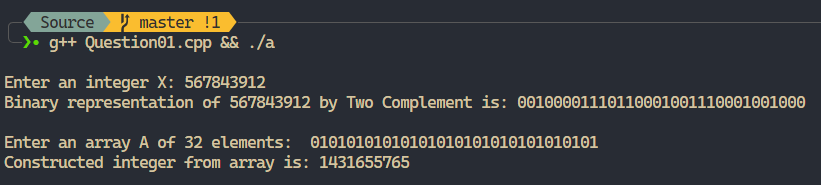
\includegraphics[width=\textwidth]{images/img1.PNG}
	\caption{Chụp màn hình kết quả bài 1.}
\end{figure}

Chương trình nhập vào số 567843912 và xuất ra dãy bit nhị phân dưới dạng bù 2 của số đó là: 00100001110110001001110001001000.

Chương trình nhập vào chuỗi bit 01010101010101010101010101010101 và xuất ra số nguyên tương ứng là: 1431655765.

\subsection{Bài 2}

Viết chương trình Nhập vào 2 dãy bit 8 bit (ở dạng bù 2):
Hãy thực hiện các phép tính cộng, trừ, nhân, chia trên 2 dãy bit đã nhập (Lưu ý: thực hiện theo thuật toán đã học).

\begin{figure}[H]
	\centering
	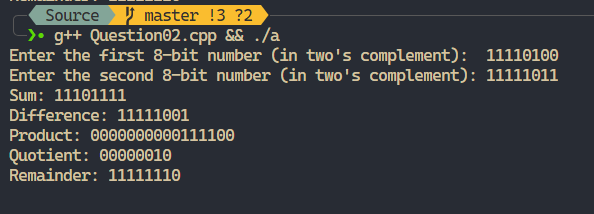
\includegraphics[width=\textwidth]{images/img2.PNG}
	\caption{Chụp màn hình kết quả bài 2.}
\end{figure}

Chương trình nhập vào 2 dãy bit 8 bit dưới dạng bù 2 là 11110100 và 11111011 tương ứng với số -12 và -5. Kết quả của các phép toán là:
\begin{itemize}
	\item Cộng: 11101111 (tương ứng với số -17).
	\item Trừ: 11111001 (tương ứng với số -7).
	\item Nhân: 0000000000111100 (tương ứng với số 60).
	\item Chia lấy thương: 00000010 (tương ứng với số 2).
	\item Chia lấy dư: 11111110 (tương ứng với số -2) do dấu của thương cùng dấu với số bị chia.
\end{itemize}
